Estudaremos agora o motor CC com excitação separada alimentado por um retificador controlado.

\subsubsection{Retificador controlado de meia onda}

As figuras \ref{fig:C1-31-II} e \ref{fig:G1-31-II} representam respectivamente o circuito e as formas de onda do retificador controlado de meia onda.
 
 \begin{figure}[ht!]
\center
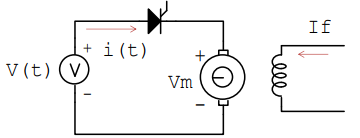
\includegraphics[scale= 0.88]{imagens/circuito1_31_II.png}
\caption{\label{fig:C1-31-II}Retificador controlado de meia onda}
\caption*{Fonte: MARTINS, cap. 6, eslaide 2.}
\end{figure}

\begin{figure}[ht!]
\center
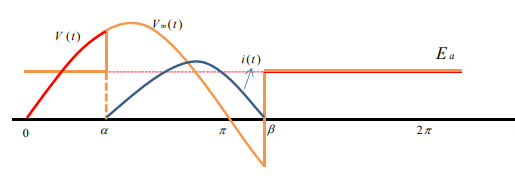
\includegraphics[scale= 0.88]{imagens/grafico1_31_II.png}
\caption{\label{fig:G1-31-II}Principais formas de onda}
\caption*{Fonte: MARTINS, cap. 6, eslaide 3.}
\end{figure}

Onde:

$V_{m}(t) \rightarrow$ tensão nos terminais da máquina.

$i(t) \rightarrow$ corrente de armadura.

$E_{a} \rightarrow$ força eletromotriz da máquina.

$v(t) \rightarrow$ tensão de alimentação.

Considerando $\omega_{m}$ constante, $E_{a}$ também será constante. A velocidade sofre uma pequena ondulação, pois o torque elétrico produzido pelo motor é pulsado. 

A tensão média nos terminais da máquina pode ser obtida a partir da seguinte expressão:
\[V_{m} = R.I_{a} + E_{a}\]
\[R.I_{a} = \frac{\sqrt{2}.V}{2\pi}\left[\cos{\alpha} - \cos{\beta} - \frac{E_{a}}{\sqrt{2}V}\left(\beta - \alpha\right)\right]\]

Logo, a expressão da característica torque velocidade é dada por:
\[\frac{R.I_{a}}{\sqrt{2}V}  = \frac{I}{2\pi}\left[\cos{\alpha} - \cos{\beta} - \frac{E_{a}}{\sqrt{2}V}\left(\beta - \alpha\right)\right]\]

Onde:

\[\frac{R.I_{a}}{\sqrt{2}V} = t_{f}\]
\[\frac{E_{a}}{\sqrt{2}V} = a\]

Para $I_{f}$ constante o torque é proporcional a $I_{a}$. Logo, $t_{f}$ é definido como fator de torque. Portanto:

\[t_{f} = \frac{1}{2\pi}\left[\cos{\alpha} - \cos{\beta} - a\left(\beta - \alpha\right)\right]\]

A expressão anterior define as características torque-velocidade do motor associado ao retificador. Assim tem-se a seguinte função: $t_{f} = f(a)$, onde $\beta$ é fixado, e $\alpha$ é um parâmetro.

\subsubsection{Retificador de meia onda com diodo de roda livre}

O emprego do diodo de roda livre aprimora o comportamento do motor. Sua estrutura está representada na figura \ref{fig:C1-32-II}

\begin{figure}[ht!]
\center
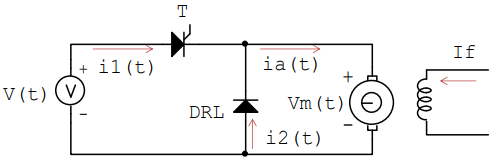
\includegraphics[scale= 0.88]{imagens/circuito1_32_II.png}
\caption{\label{fig:C1-32-II} Retificador de meia onda com roda livre}
\caption*{Fonte: MARTINS, cap. 6, eslaide 6.}
\end{figure}

E as formas de onda estão ilustradas na fig \ref{fig:C1-32-III}

\begin{figure}[ht!]
\center
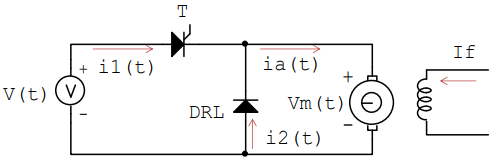
\includegraphics[scale= 0.88]{imagens/circuito1_32_II.png}
\caption{\label{fig:C1-32-III} Principais formas de onda}
\caption*{Fonte: MARTINS, cap. 6, eslaide 6.}
\end{figure}

Neste caso:

\[i_{1} = \frac{\sqrt{2}V}{R}\left\{\cos{\theta}\sin\left(\omega{t} - \theta\right) - a + \left[a - \cos{\theta}\sin{\left(\alpha - \theta\right)}\right]e^{-\left(\omega{t} - \alpha\right)/\tan{\theta}}\right\}\]

\[i_{2}(t) = i_{1}(\pi)e^{-\frac{\omega{t}}{\tan{\theta}}} - \frac{E_{a}}{R}\left(1 - e^{-\frac{\omega{t}}{\tan{\theta}}}\right)\]

Quando $\omega{t} = \beta \Rightarrow i_{2}(t) = 0$. Assim, levando essa conclusão nas equações anteriores tem-se que:
\[\beta = \tan{\theta}.ln\left[\frac{R.i_{1}(\pi)}{E_{a}} + 1\right]\]

O valor da tensão média nos terminais do motor é dado abaixo:

\[V_{m} = E_{a} - \frac{(\beta - \alpha)}{2\pi}E_{a} + \frac{\sqrt{2}V}{2\pi}\left(1 + \cos{\alpha}\right)\]

Onde:
\[V_{m} = R.I_{a} + E_{a} \Rightarrow R.I_{a} = V_{m} - E_{a}\]

Logo,
\[R.I_{a} = \frac{\sqrt{2}V}{2\pi}\left[1 + \cos{\alpha} - \frac{E_{a}}{\sqrt{2}V}\left(\beta - \alpha\right)\right]\]

Definindo $t_{f} = \frac{R.I_{a}}{\sqrt{2}V} \rightarrow$ fator torque, obtém-se:

\[t_{f} = \frac{1}{2\pi}\left[1 + \cos{\alpha} - a\left(\beta - \alpha\right)\right]\]

A partir desta equação é possível determinar a característica torque-velocidade do motor CC.

\subsubsection{Retificador misto de onda completa com diodo de roda livre}

A estrutura de potência do retificador misto de onda completa com diodo de roda livre alimentando o motor CC é apresentado na figura \ref{fig:C1-33-II}

\begin{figure}[ht!]
\center
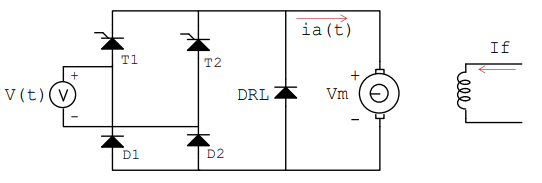
\includegraphics[scale= 0.88]{imagens/circuito1_33_II.png}
\caption{\label{fig:C1-33-II} Retificador misto de onda completa com diodo de roda livre}
\caption*{Fonte: MARTINS, cap. 6, eslaide ARRUMAR.}
\end{figure}

Esta estrutura é uma das mais empregadas industrialmente para motores CC até 10 KW. É econômica por conter somente dois tiristores. A presença do diodo $D_{RL}$, aliada à retificação de onda completa contribui para a redução das harmônicas de corrente de armadura e para minimizar os problemas ligados à condução descontínua. As de formas de onda, para condução descontínua e contínua, são apresentadas nas figuras \ref{fig:G1-33-II} e \ref{fig:G2-33-II}

\begin{figure}[ht!]
\center
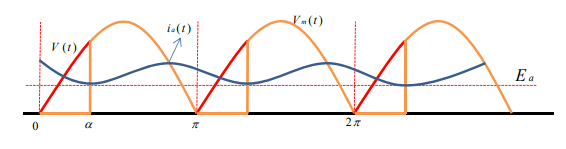
\includegraphics[scale= 0.88]{imagens/grafico1_33_II.png}
\caption{\label{fig:G1-33-II} Principais formas de onda para condução contínua}
\caption*{Fonte: MARTINS, cap. 6, eslaide ARRUMAR.}
\end{figure}

\begin{figure}[ht!]
\center
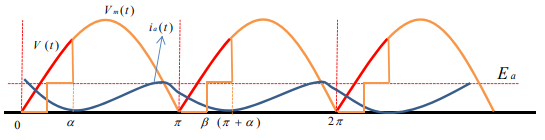
\includegraphics[scale= 0.88]{imagens/grafico2_33_II.png}
\caption{\label{fig:G2-33-II} Principais formas de onda para condução descontínua}
\caption*{Fonte: MARTINS, cap. 6, eslaide ARRUMAR.}
\end{figure}

Quando o tiristor conduz, a tensão nos terminais do motor é igual a tensão da rede. Durante a roda livre a tensão é nula, e durante a descontinuidade a tensão nos terminais da máquina é a própria força contra eletromotriz do motor.


\subsubsection{Equacionamento básico}

\[i_{1} = \frac{\sqrt{2}V}{R}\left\{\cos{\theta}\sin\left(\omega{t} - \theta\right) - a + \left[a - \cos{\theta}\sin{\left(\alpha - \theta\right)}\right]e^{-\left(\omega{t} - \alpha\right)/\tan{\theta}}\right\}\]

\[i_{2}(t) = i_{1}(\pi)e^{-\frac{\omega{t}}{\tan{\theta}}} - \frac{E_{a}}{R}\left(1 - e^{-\frac{\omega{t}}{\tan{\theta}}}\right)\]

\[\beta = \tan{\theta}.ln\left[\frac{F_{1}(\theta,a,\alpha,\pi)}{a} + 1\right]\]

Sendo $F_{1}(\theta,a,\alpha,\pi) = \cos{\theta}\sin\left(\pi - \theta\right) - a + \left[a - \cos{\theta}\sin{\left(\alpha - \theta\right)}\right]e^{-\left(\pi - \alpha\right)/\tan{\theta}} $.

Deseja-se, estabelecer as características torque-velocidade do motor. Assim:

\begin{itemize}
    \item Condução descontínua:
	\[t_{f} = \frac{1}{\pi}\left[1 + \cos{\alpha} - a(\beta - \alpha)\right]\]
    \item Condução contínua:
	\[t_{f} = \frac{1}{\pi}\left[1 + \cos{\alpha} - \pi{a}\right]\]
\end{itemize}

A condução é crítica quando $\beta = \pi + \alpha$. Portanto, a partir da seguinte expressão:

\[\beta = \tan{\theta}.ln\left[\frac{F_{1}(\theta,a,\alpha,\pi)}{a} + 1\right]\]

Obtém-se:

\[\pi + \alpha = \tan{\theta}.ln\left[\frac{F_{1}(\theta,a,\alpha,\pi)}{a} + 1\right]\]

Logo, sabendo a e $\alpha$, pode-se determinar $\theta$; e consequentemente pode-se determinar a indutância crítica:

\[\tan{\theta_{c}} = \frac{\omega.L_{c}}{R}\]
\[L_{c} = \frac{R}{\omega}\tan{\theta_{c}}\]

